\chapter{Development Progress}
\label{chap:developmentprogress}
Figure \ref{fig:timeline-dev-progress} illustrates the proposed timeline for the KU Parking Project, which includes collecting the dataset and initiating the Car Detection Model in this semester.

\begin{figure}[H]
    \centering
    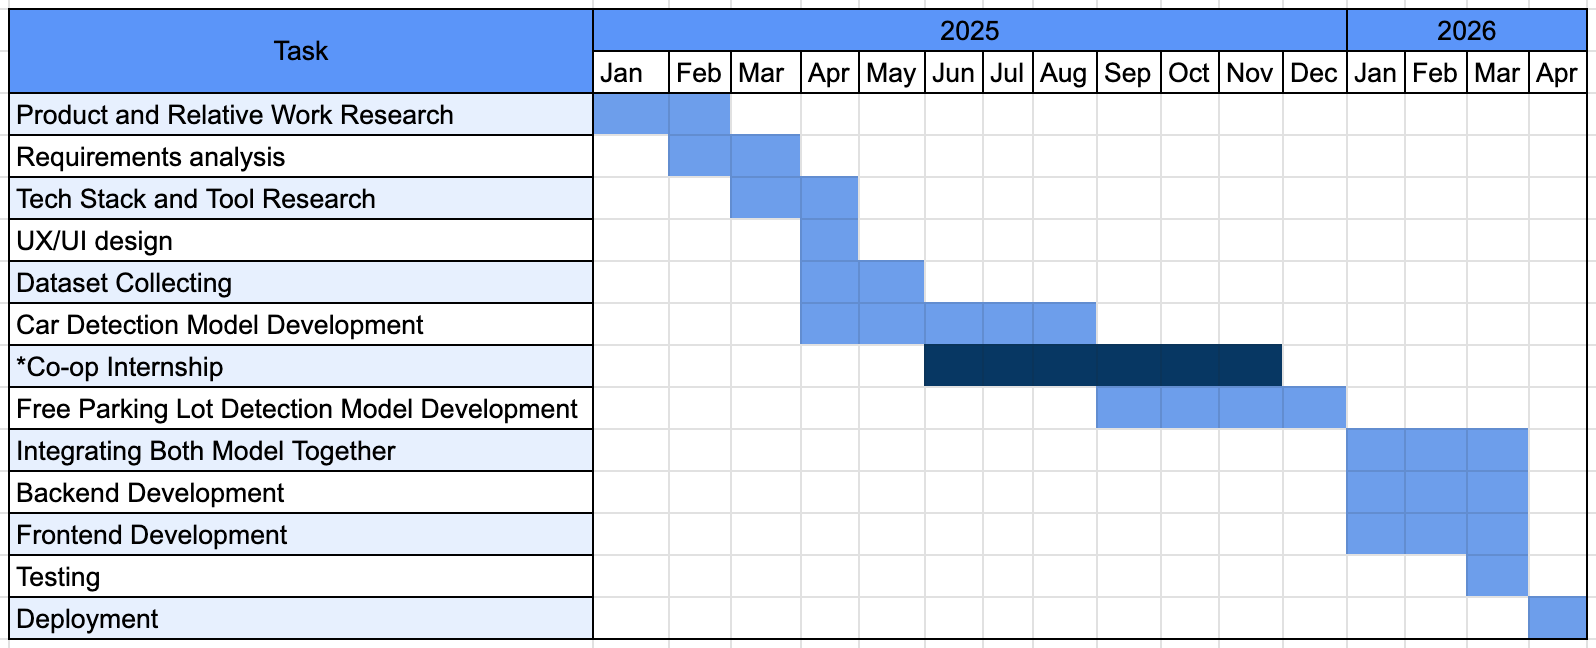
\includegraphics[width=\textwidth,height=0.5\textheight,keepaspectratio]{timeline/KU-Parking_timeline.png}
    \caption{Proposed Timeline for KU Parking Project}
    \label{fig:timeline-dev-progress}
\end{figure}

\section{Modules Developed}
\label{section:module-developed}
In this semester, we worked on the Car Detection Model, which includes the following files:
% TODO: Add Module Explanation

\section{Screenshot}
\label{section:screenshot}
\begin{figure}[H]
    \centering
    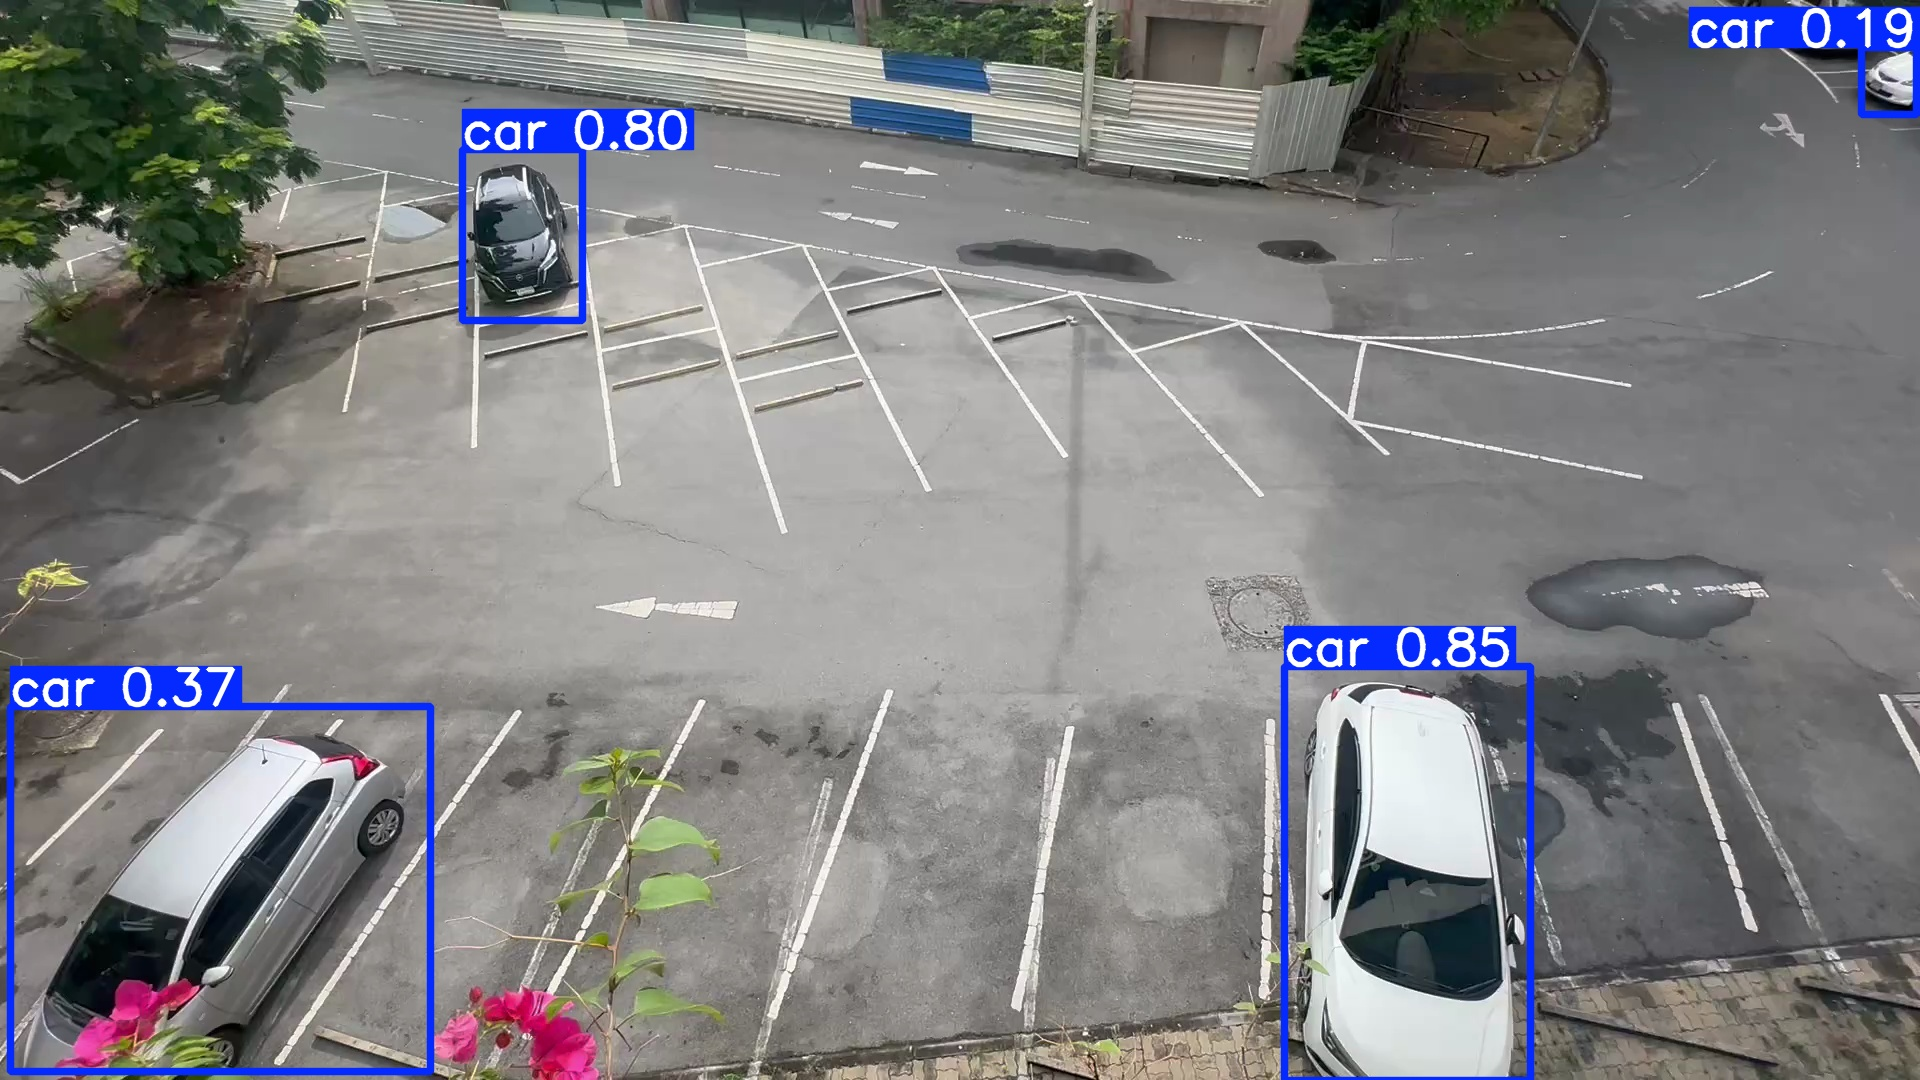
\includegraphics[width=\textwidth,height=0.5\textheight,keepaspectratio]{screenshot/screenshot_001.jpg}
    \caption{Screenshot of detection model on Computer Department Parking Area}
    \label{fig:screenshot001}
\end{figure}


\section{Experimental Results}
\label{section:experimental-results}
The outcome of this semester’s development is the first version of our Car Detection Model. The source code is available in our \href{https://github.com/ReggieReo/ku-parking-ai-component}{GitHub repository} or can be accessed by scanning the QR code in Figure~\ref{fig:github-repo-ai-component-qr}.
\begin{figure}[H]
    \centering
    
\includegraphics[width=\textwidth,height=0.5\textheight,keepaspectratio]{misc/github-repo-qr.png}
    \caption{QRcode for KU Parking AI Component Repository}
    \label{fig:github-repo-ai-component-qr}
\end{figure}

\section{Datasets}
\label{section:datasets}
We've modified our dataset collection method. Due to the semester break in mid-April, footages captured from the Computer Department Parking Facility contained a limited number of cars, resulting in a less diverse dataset. To improve the variety and robustness of our car detection dataset, we supplemented it with online footage sources to our train dataset.

For access to the dataset, please visit our Google Drive \href{https://drive.google.com/drive/folders/1pOUgcbsFb1mpLc5oywZ2xQdRepm_nVu7?usp=sharing}{Link} or scan Figure \ref{fig:dataset-qr}
\begin{figure}[H]
    \centering
    
\includegraphics[width=\textwidth,height=0.5\textheight,keepaspectratio]{misc/dataset_qr.png}
    \caption{QRcode for KU Parking Dataset}
    \label{fig:dataset-qr}
\end{figure}

\section{Gantt chart}
\label{section:gantt-chart}
As of May 2025, the current timeline for the KU Parking Project is depicted in Figure \ref{fig:11-05-25-timeline-dev-progress}.
\begin{figure}[H]
    \centering
    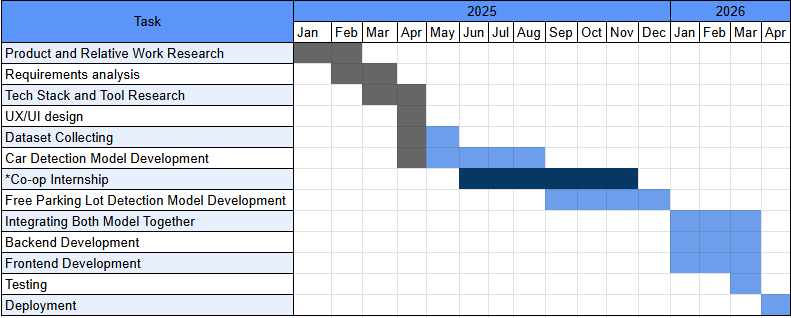
\includegraphics[width=\textwidth,height=0.5\textheight,keepaspectratio]{timeline/11-05-25-KU-Parking-timeline.PNG}
    \caption{Updated Timeline for KU Parking Project}
    \label{fig:11-05-25-timeline-dev-progress}
\end{figure}

\section{Self-evaluation}
\label{section:self-evaluation}
As mentioned in the Datasets section (Section \ref{section:datasets}), we have modified our dataset collection approach. This has led to minor adjustments and re-planning during the data collection phase. Model development remains on schedule; however, we anticipate that the upcoming Cooperative Internship period, spanning from June to November, may affect the development pace. Consequently, further development of the Parking Lot Detection Model may be postponed to January 2026. In the worst-case scenario—if the Car Detection Model is not completed before the end of January 2026—we may need to consider cutting the Parking Lot Detection Model and shifting focus to software-side development.